\documentclass[12pt]{article}
\usepackage{amsfonts, epsfig}
\usepackage{amsmath}
\usepackage{graphicx}
\usepackage{fancyhdr}
\pagestyle{fancy}
\lfoot{\texttt{timmulvaney.github.io}}
\lhead{Tim Mulvaney Introduction to AI - Coursework}
\rhead{\thepage}
\cfoot{}

% import biblatex package
\usepackage[backend=biber]{biblatex}
\addbibresource{file.bib}

\begin{document}


\section*{Question 1 - Visualization and Analysis of Penguin Dataset}

The Pengiun dataset \cite{PM} contains data relating to the Adelie, Chinstrap and Gentoo penguins
There are two categorical input variables
information about penguins of one of three types. You task is to
explore the dataset and to predict the penguin type. The dataset is
known as the Palmer Penguins and can be found at:\\
\\
\texttt{allisonhorst.github.io/palmerpenguins/}\\
\\
This link contains information on how to cite the dataset.


The problem is one of classification as the species is categorical (. 
The problem can be converted to one of regression?


You should consider how to visualize the data and which algorithms to
try. Nothing you do will be completely successful, this coursework is
not here to judge your final accuracy but the care you bring to your
investigation. Here are some thing you should consider:
\begin{itemize}
  \item The kind of algorithm to use, for example whether to classify, regress  or cluster.
  \item The metric to use to measure the performance of the model.
  \item What sort of baseline to compare the model to.
  \item How to choose the hyperparameters of your model.
\end{itemize}
For good marks you should include some graphs that illustrate
properties of the data and you should compare two classification
algorithms, both to each other and to a baseline model. The algorithms
you pick do not need to be unusual, for example $k$nn classification
would be perfectly good, though, of course, for full marks this would
include some consideration of how to pick $k$ and how to measure the
distance, though, as you know, no approach to chosing $k$ is every
going to be completely satisfactory. In addition, you should include
either some exploratory regression or unsupervised learning; for
regression you might regress two properties and examine whether the
regression parameters are the same for each penguin type; unsupervised
learning could use $k$-means, for example. You do not need to do both
regression and unsupervised learning.

You should make sure any assessment is not restricted to the data used
in train models or decide on metaparameters. In your report you should
explain your decisions. You code will not be marked for elegance, but
it should run correctly; it is expected you will use Python, but any
of Python, Julia or R is fine. Do not include screenshots of graphs,
they should be imported directly; resize them to the correct size
before importing them, if the labels are tiny the graphs will not be
marked. Make sure figure captions are descriptive, it is better to
have some overlap between figure captions and the main text than to
have figure captions that are not reasonably self-contained.

As a rough guide to marking:
\begin{itemize}
\item Initial description of the data, including some graphs or other approaches to visualisation. 6 marks.
\item Either unsupervised learning or regression. 6 marks.
\item Two algorithms should be tested, if only one algorithm is
  included the 28 available marks will be halved.
\item Overall presentation (3 marks), including use of appropriate
  sections, plots, diagrams, or tables to make your point. Do not
  include code snippets in the report. Instead, describe in words or
  equations what you are implementing. Format equations correctly.
\item Suitable choice of algorithms (4 marks).
\item Suitable choice of evaluation for algorithms (3 marks).
\item Comparison with a suitable baseline (3 marks) and a justification for which baseline to use.
\item A description of metaparameter selection (3 marks), if one
  algorithm has not metaparameter, then explain that and note why not
  and why this do or does not make it a better algorithm for these
  data.
\item Describe and compare the results from your two algorithms,
  include a description of how you implemented the algorithms. (6 marks)
\item There are some marks (6 marks) for something suprising and unusual.
\end{itemize}




\section*{Question 2 - Ethical challenge facing us in data science and AI}

For two of these three types of ethical challenge facing us in data science and AI:
\begin{enumerate}
\item The protection of data, of the people whose data they are and participants in any study.
\item Avoiding the amplification of biases and regressive values implicit in historic dataset.
\item The safety of AI systems and the possible of existential threats from machines.
\end{enumerate}
describe what you think is a specific example of a challenge that
could arise or has arisen in the past. Obviously the three broad types
of challenge overlap, do not worry about the boundaries between these
types, but do try to address different types of threat in your
examples. Explain how the ethical problems could be addressed, or at
least made more transparent.

\subsection*{Report}

Your report should be no longer than five pages, including any
references. It is expected that Question 2 would occupy about a fifth
of this space; use an 11 or 12pt font and do not try tricks like
expanding the margin to fit in more text, shorter is better than
longer.

Your report must be submitted in pdf and should be prepared in LaTeX;
overleaf is a good approach, but not required as long as LaTeX has
been used. As always when using LaTeX, give yourself over to defaults,
our expectation of what a document should look like has been
conditioned on LaTeX, so it is best not to try to override the look of
the document.

Avoid code snippets in the report unless that feels like the best way
to illustrate some subtle aspect of an algorithm; do always though
consider a mathematical description if possible. You will be asked to
submit code and it may be tested to make sure it works and matches
your report. It will not, however, be marked in and of itself.

\subsection*{knn}

Perhaps use F1-score (there are others!) as the classes are imbalanced in number?

F1-score is a metric that considers both precision and recall. Precision measures the accuracy of positive predictions (TP/(TP+FP)), while recall (also known as sensitivity) measures the fraction of positives that were correctly identified (TP/(TP+FN))
F1-score is the harmonic mean of precision and recall and is calculated as follows:
F1 = 2x(PrecisionxRecall)/(Precision+Recall)
F1-score ranges from 0 to 1, where a higher value indicates better model performance. F1-score is particularly useful when classes are imbalanced because it considers both false positives and false negatives.


\section*{Report template}

This is a report template, you don't need to use this template, but do
use it if it is helpful.


Here is an example of an equation:
\begin{equation}
  \pi=4\left(1-\frac{1}{3}+\frac{1}{5}-\frac{1}{7}\ldots\right)
\end{equation}
or
\begin{equation}
  \pi=4\sum_{n=0}^\infty\frac{(-1)^{n}}{2n+1}
\end{equation}
where $\pi$ can be written in line by using \$'s. Here is a vector:
\begin{equation}
\mathbf{x}=\left(\begin{array}{c}x_1\\x_2\end{array}\right)
\end{equation}

You can write in \textbf{bold}, or \textsl{italics} or \texttt{true
  type}, often the latter is used for specific commands or libraries in a
programming language, as in `I used \texttt{numpy} v1.23.4 to\ldots'. Notice the use of the left quote symbol found in the top left of the keyboard to get the left quote. There is also blackboard bold often used for things like $\mathbb{R}$ for real numbers and there is calligraphic for fancy things like $\mathcal{L}$ but this is becoming increasing irrelevant to what you are likely to need! 

There is a table at Table~\ref{tab:example} and a figure at Fig.~\ref{fig:example}.

\begin{table}
\begin{center}
\begin{tabular}{l|cc}
colour&size&weight\\
\hline
blue&12&14\\
red&8&25
\end{tabular}
\end{center} 
\caption{\textbf{An example table}. You need to specify the number of columns and how the text is justified, left, right or center. Each line ends in a double backslash and an ampersand, \&, separates each column.}
\label{tab:example}
\end{table} 

% \begin{figure}
% \centering
% 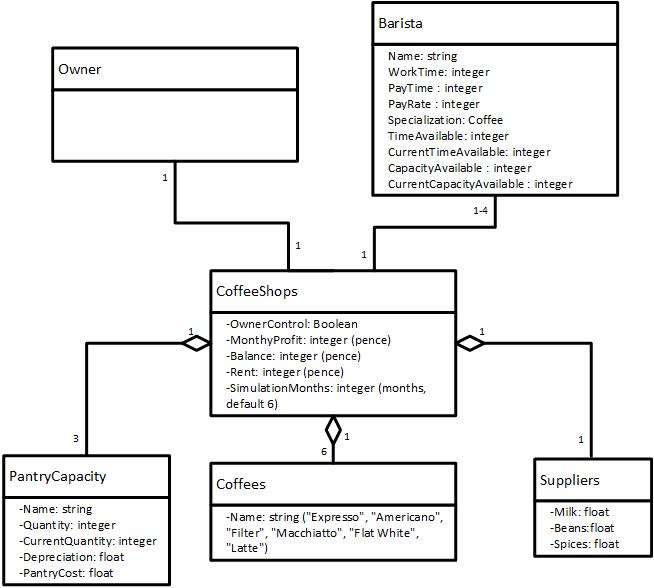
\includegraphics[width=0.8\textwidth,natwidth=610,natheight=642]{UML.jpg}
% \caption{\textbf{An example figure}. Figure example}
% \label{fig:example}
% \end{figure}

\begin{figure}[ht!]
\centering
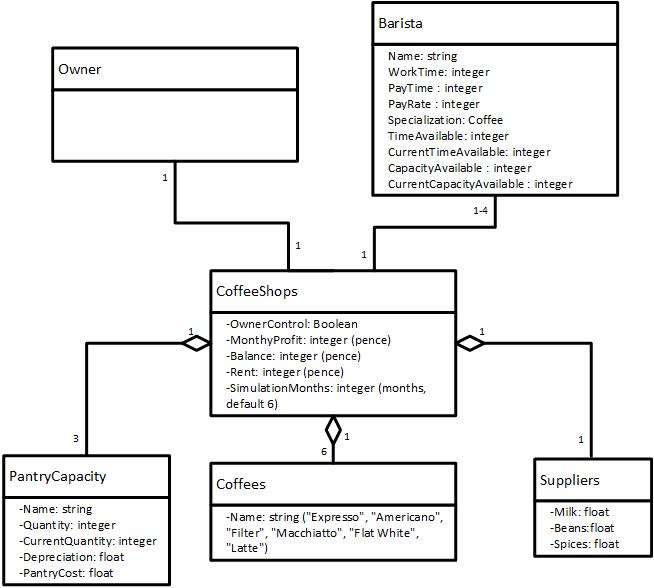
\includegraphics[width=90mm]{UML.jpg}
\caption{A simple caption \label{fig:example}}
\end{figure}


\printbibliography

\end{document}
